\documentclass{beamer}

\usepackage{lmodern}
\usepackage[utf8]{inputenc}
\usepackage{hyperref}
\usepackage{tabularx}
\usepackage{siunitx}
\usepackage{todonotes}
\sisetup{output-exponent-marker=\ensuremath{\mathrm{e}}}

\usetheme{Madrid}
\usecolortheme{default}

%------------------------------------------------------------
\title[About Beamer]
{About the Beamer class in presentation making}

\subtitle{A short story}

\author[Claudio, Jos\'e]
{Claudio Scheer\inst{1} \and Jos\'e Fernando Possebon\inst{1}}

\institute[PUCRS]
{
  \inst{1}%
  Pontifical Catholic University of Rio Grande do Sul - PUCRS\\
  \{claudio.scheer, jose.possebon\}@edu.pucrs.br
}

\date[Deep Learning 2020]
{Deep Learning, June 2020}


\AtBeginSection[]
{
  \begin{frame}
    \frametitle{Table of Contents}
    \tableofcontents[currentsection]
  \end{frame}
}
%------------------------------------------------------------


\begin{document}

\frame{\titlepage}


%---------------------------------------------------------
\begin{frame}
  \frametitle{Table of Contents}
  \tableofcontents
\end{frame}
%---------------------------------------------------------


%---------------------------------------------------------
\section{Proposal}

\begin{frame}
  \frametitle{Proposal}

  % \begin{itemize}
  %   \item<1-> Text visible on slide 1
  %   \item<2-> Text visible on slide 2
  %   \item<3> Text visible on slides 3
  %   \item<4-> Text visible on slide 4
  % \end{itemize}
\end{frame}

% \begin{frame}
%   In this slide \pause

%   the text will be partially visible \pause

%   And finally everything will be there
% \end{frame}
%---------------------------------------------------------


%---------------------------------------------------------
\section{Dataset}

\begin{frame}
  \frametitle{The Enron Email Dataset}

  {\scriptsize
    no, i dont mind.       : - )
    \bigbreak
    -----Original Message-----
    \bigbreak
    Hi how are you doing?  I have a meeting from 4 to 5, do you mind waiting for me?  Thanks.

    John
    \bigbreak
    -----Original Message-----
    \bigbreak
    hello
  }
\end{frame}

\begin{frame}
  \frametitle{The Enron Email Dataset}

  {\scriptsize
    yuck yuck
    \bigbreak
    -----Original Message-----
    \bigbreak
    har har
  }
  \bigbreak
  \bigbreak

  The subject is: \textbf{Wine tasting}.
\end{frame}

\begin{frame}
  \frametitle{The Enron Email Dataset}

  \begin{itemize}
    \item \href{https://www.kaggle.com/claudioscheer/extract-reply-emails}{https://www.kaggle.com/claudioscheer/extract-reply-emails};
    \item Get only emails with less than 256 characters;
  \end{itemize}

  \bigbreak
  \bigbreak
  \bigbreak

  Final dataset: \num{40062} input-target pairs.
  \\
  Train dataset: \num{10002} input-target pairs.
\end{frame}

\begin{frame}
  \frametitle{Samples}

  \begin{table}
    \centering
    \begin{tabularx}{\textwidth}{|X|X|}
      \hline
      \textbf{Input}                                                            & \textbf{Target}                                                                       \\
      \hline
      I thought this one was canceled. So I declined to get it off my calendar. & You're right.                                                                         \\
      \hline
      Rex - thanks for the quick response...please note the revised letters below.
      Previous email had a clerical error                                       & Who will sign theses?                                                                 \\
      \hline
      Where can I get info on safety statistics for the pipes?                  & Ralph, please get with Rod and provide what ever he needs in the way of Safety Stats. \\
      \hline
    \end{tabularx}
  \end{table}
\end{frame}
%---------------------------------------------------------


%---------------------------------------------------------
\section{BERT}

\begin{frame}
  \frametitle{BERT architecture}

  \todo[inline]{Describe here the architecture that the professor showed in the class.}
\end{frame}

\begin{frame}
  \frametitle{Hugging Face}

  \begin{itemize}
    \item BERT base was used;
          \begin{itemize}
            \item 12 layers;
          \end{itemize}
    \item Hugging Face and PyTorch was used;
  \end{itemize}
\end{frame}

\begin{frame}
  \frametitle{Learning rate schedule}

  \begin{itemize}
    \item Warm-up steps: \num{5000};
    \item Learning rate: \num{1e-4};
  \end{itemize}

  \bigbreak
  \bigbreak

  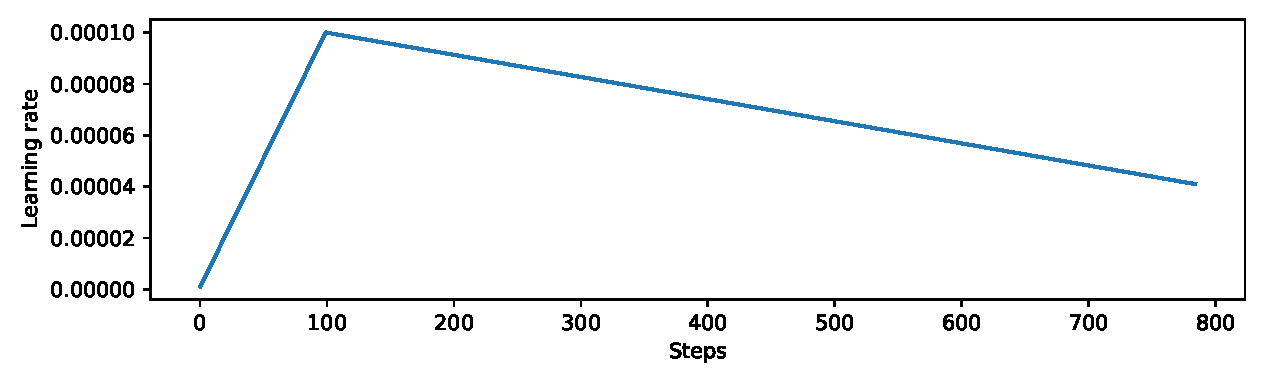
\includegraphics[width=\textwidth]{../images/warmup_linear_schedule.pdf}
\end{frame}

\begin{frame}
  \frametitle{Optimizer and hyperparameters}

  \begin{itemize}
    \item Adam;
          \begin{itemize}
            \item Adam epsilon: \num{1e-4};
          \end{itemize}
    \item Batch size: \num{10};
    \item Training epochs: \num{10.5};
    \item Beam search hypothesis: \num{3};
  \end{itemize}
\end{frame}

\begin{frame}
  \frametitle{Loss function}

  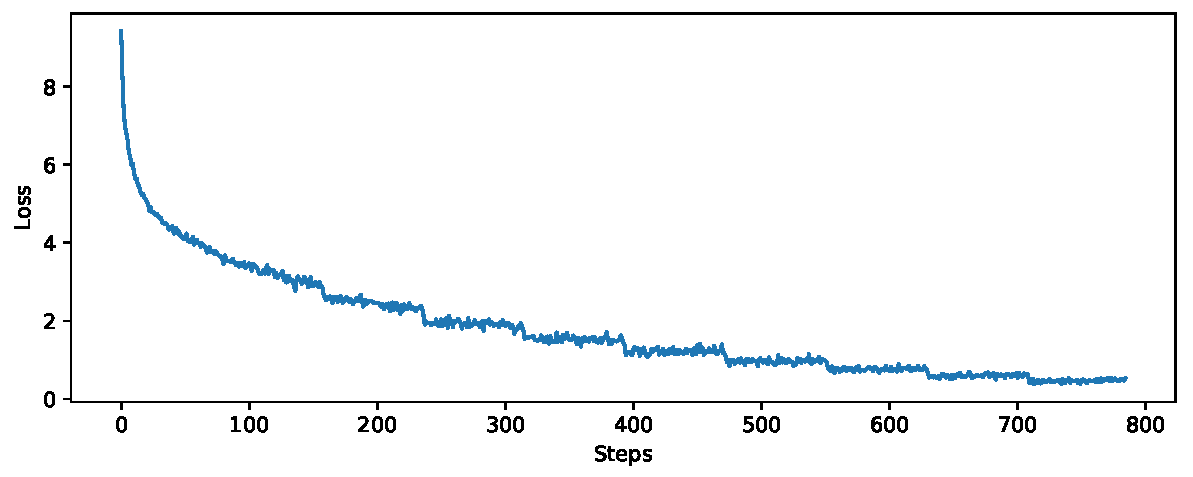
\includegraphics[width=\textwidth]{../images/loss_function.pdf}
\end{frame}
%---------------------------------------------------------


%---------------------------------------------------------
\section{Results}

\begin{frame}
  \frametitle{BLEU score}

  \begin{itemize}
    \item <1-> 21 emails in the evaluation dataset;
    \item <2-> BLEU score = \num{0.0};
  \end{itemize}
\end{frame}

\begin{frame}
  \frametitle{BLEU score}

  \begin{table}
    \begin{tabularx}{\textwidth}{|X|X|X|}
      \hline
      \textbf{Input}                                                  & \textbf{Target}                                          & \textbf{Generated}                                                                                                           \\
      \hline
      nevermind.  are you at work?                                    & yea                                                      & i'm all alone over here...                                                                                                   \\
      \hline
      what re your plans for tomorrow?                                & drop prentice's car off at shop; go to dome              & leaving early tomorrow. leaving early. leaving early. leaving early.                                                         \\
      \hline
      I just refaxed it.  For your information, my total hours is 49. & I noted your hours..I will look for the t/s Thanks Lisa! & Thanks Rick, and let's talk after the holidays about a new game plan... Best regards and happy thanksgiving. Jaime Williams. \\
      \hline
    \end{tabularx}
  \end{table}
\end{frame}

\begin{frame}
  \frametitle{Generated replies}

  \begin{table}
    \scriptsize
    \begin{tabularx}{\textwidth}{|X|X|c|c|}
      \hline
      \textbf{Email}                                                                                                                                                                                        & \textbf{Reply}                                                                                                                                                                                                                     & \textbf{AI?} & \textbf{Correct?} \\
      \hline
      Let me know if this works.                                                                                                                                                                            & This works great. Will let you know. as soon as I get a chance, let me know                                                                                                                                                        & \num{0}{\%}  & yes               \\
      \hline
      Following are the terms under which I ran the Forward Obligation report and received this message: General SQL error. ORA-00907: missing right parenthesis. Terms: Let me know what you find. Thanks! & Kate, I ran the report with the exact same options and it came right up. Try it again, exactly as before. Usually if it works for one person and not the other it is a security issue. Let me know what happens. Thanks, Brettther & \num{0}{\%}  & yes               \\
      \hline
      Didn't you trade uranium at one time?                                                                                                                                                                 & Yeah, I know the buisness VERY well.                                                                                                                                                                                               & \num{0}{\%}  & no                \\
      \hline
      Are you free for drinks either Monday or Wednesday?                                                                                                                                                   & Yes                                                                                                                                                                                                                                & \num{0}{\%}  & no                \\
      \hline
      Mons, I would be available on the 25th, 26th or 27th. I cannot make it the week of the 18th. Thanks, Bill.                                                                                            & OK, so, let's see if we can get together later today. I have to leave at 16:00 for a few minutes, but I am sure that I will be out at that moment. Thank you Kim.                                                                  & \num{0}{\%}  & yes               \\
      \hline
    \end{tabularx}
  \end{table}
\end{frame}
%---------------------------------------------------------


%---------------------------------------------------------
\section{Miscellaneous}

\begin{frame}
  \frametitle{Miscellaneous}

  \begin{itemize}
    \item \href{https://github.com/claudioscheer/seq2seq-bert}{https://github.com/claudioscheer/seq2seq-bert};
    \item \href{https://github.com/claudioscheer/seq2seq-bert/releases/tag/v0.0.8-alpha}{Final release (v0.0.8)};
  \end{itemize}
\end{frame}
%---------------------------------------------------------

\end{document}